% The Yang--Mills mass gap, read through DMP. Draft of 21 November 2026.
% Build: pdflatex mass-gap.tex twice (bibliography inline). Figures: python figures.py. Checks: python checks.py.
\documentclass[11pt,a4paper]{article}
\usepackage[T1]{fontenc}
\usepackage[utf8]{inputenc}
\usepackage{lmodern}
\usepackage[margin=2.5cm]{geometry}
\usepackage{amsmath,amssymb,amsthm}
\usepackage{booktabs,tabularx,array}
\usepackage{enumitem}
\usepackage{graphicx}
\usepackage[hidelinks]{hyperref}
\usepackage{url}
\setlength{\emergencystretch}{3em}
\newcolumntype{L}{>{\raggedright\arraybackslash}X}
\newcommand{\lean}[1]{\texttt{#1}}
\newcommand{\pending}[1]{\textbf{[pending: #1]}}
\newtheorem*{lemma}{Lemma}

\title{The Yang--Mills mass gap, read through a trust protocol\\[0.6ex]
\large A dictionary and its limits, pre-registered lattice tests, and an independent formal proof of the strong-coupling area law}
\author{Steven Hrovat\thanks{Independent. Contact: \href{mailto:hrovat.steven@googlemail.com}{\nolinkurl{hrovat.steven@googlemail.com}}.}
\and Claude (Anthropic)\thanks{An AI system (Claude Opus 5.5) working in the first author's sessions. See ``Contributions and use of AI''.}}
\date{Draft of 21 November 2026}

\begin{document}
\maketitle

\begin{abstract}
\noindent The Yang--Mills mass gap problem asks for a proof that the quantum theory of the strong force, built without any mass in its
equations, nevertheless has a smallest positive energy. We read the problem through DMP, an axiom system for trust in distributed software,
and report what that reading does and does not deliver. It delivers a dictionary: a trust network in which every part keeps its own keys
is, exactly, a lattice gauge field, and we prove the structural parts in Lean. It delivers a filter: any argument that would also give the
photon a mass is wrong, and this rules out every gap mechanism DMP's text offers. And it delivers a restatement: in DMP's terms the gap is
a bound on how far an act of the strong force can reach, the same at every scale; in physics that bound is the gap itself, so the
restatement locates the open problem and does not solve it. Around this reading we ran five pre-registered lattice tests on our own code
(SU(2) and U(1) in four dimensions, on a laptop GPU), and we report every verdict, including three failures, two of them followed up by
separately pre-registered checks. Independently of DMP, we give a Lean proof of the strong-coupling area law for SU(2) and U($n$) lattice
gauge theory (confinement at very small coupling, known since 1978; formalised before us by others, by a different route), and sharper
single-link bounds for the Dobrushin argument of the \texttt{lgt} Lean library. We do not claim a proof of the mass gap, and nothing here is one.
\end{abstract}

\tableofcontents
\bigskip

%=====================================================================================================================================
\section{Introduction}\label{sec:intro}

\paragraph{The problem.} A quantum field theory has a \emph{mass gap} if every excitation of its vacuum costs at least some fixed energy
$\Delta>0$. Equivalently, correlations fall off exponentially with distance: a disturbance has a finite range $\xi=\hbar c/\Delta$, the
\emph{correlation length}. Light has no gap (radio waves can be arbitrarily long and cheap). The strong force is expected to have one: its
force carriers, gluons, never travel alone, and the lightest thing that does, a \emph{glueball}, has a definite mass. The Clay problem
asks for a mathematical proof of this for four-dimensional Yang--Mills theory with a compact simple gauge group~\cite{jaffewitten}.

Physicists compute on a grid (a \emph{lattice}) of spacing $a$. On any grid a gap is free, since there is always a smallest step. The
problem is whether the gap survives the limit $a\to0$ in physical units: measured in grid steps the gap $a\Delta$ must go to zero, measured
in physical units it must stay put. Two ends of this are proven. At \emph{strong coupling} (a coarse grid, in a sense made precise below)
lattice Yang--Mills has a gap and confines~\cite{os78,szz,lgt}. At the short-distance end, a 2026 Lean-checked construction shows that a
continuum Yang--Mills theory exists as a limit of lattices~\cite{openai2026}; its assessors state that it ``provides no evidence for or
against a mass gap''. The open piece is the bridge between the two: control of the theory through the middle range of scales, where the
coupling is neither small nor large.

\paragraph{What DMP is, and why read the problem through it.} DMP (the Dark Matter Protocol, version~0.9.9~\cite{dmp}) is the first author's
axiom system for a distributed software platform: it fixes how parts trust each other, how information moves between them, and what may
exist inside the system. A companion series of papers (GUID) reads these axioms as physics; its standing verdict is that DMP \emph{cannot
model} our universe but \emph{can host} physical theories as content~\cite{guidv7}. DMP's strength is transfer between fields: a problem
that looks hopeless in one vocabulary can become tractable in another. This paper tests that strength on the mass gap. The reading has to
pass one hard filter: four-dimensional lattice light (U(1)) is massless at weak coupling~\cite{guth,fs82}, so \emph{any argument that would
also give light a mass is wrong}. We call this the \emph{photon test}.

\paragraph{Contributions.}
\begin{enumerate}[nosep,leftmargin=*]
\item A dictionary between DMP and lattice gauge theory, with its structural parts proved in Lean, and an analysis of which DMP mechanisms
      pass the photon test (\S\ref{sec:dmp}). None of DMP's gap \emph{mechanisms} does; DMP's \emph{classification} of the forces does, with
      stated limits.
\item The first author's reading of the gap as a bounded reach (equivalently a bounded ``time to live'' of existence), formalised as a
      one-line consequence of two postulates, and the reason it is a restatement rather than a derivation (\S\ref{sec:reach}).
\item The layer-by-layer zoom-out computed in its simplest exact form, showing quantitatively why a layered argument fails the photon
      test unless it controls effects of size $10^{-11}$ per layer (\S\ref{sec:layers}).
\item Five pre-registered lattice tests, all verdicts reported (\S\ref{sec:lattice}), on a validated laptop-GPU code.
\item Two formal results independent of DMP (\S\ref{sec:formal}): a Lean proof of the strong-coupling area law for SU(2) and U($n$), and
      sharper single-link influence bounds for the \texttt{lgt} library's Dobrushin argument.
\end{enumerate}

\paragraph{Claim level.} Every theorem named here is checked by Lean's kernel, and every number is reproduced by the scripts in the
repository. Our lattice results reproduce known physics; they add nothing to what decades of lattice work have established. The area law
and the influence bounds are strong-coupling results, far from the physical regime. Nothing here has been reviewed by a physicist or a
mathematician. \textbf{We do not claim a proof of the Yang--Mills mass gap.}

%=====================================================================================================================================
\section{Vocabulary}\label{sec:vocab}

The paper needs about twenty terms. Table~\ref{tab:vocab} gives each in one line; the text repeats the essential ones where they are used.

\begin{table}[h]\centering\small
\caption{Vocabulary. Upper part: lattice gauge theory. Lower part: DMP.}\label{tab:vocab}
\begin{tabularx}{\linewidth}{@{}>{\raggedright\arraybackslash}p{3.3cm}L@{}}\toprule
lattice, link, plaquette & a periodic grid $(\mathbb Z/N\mathbb Z)^d$; a \emph{link} joins neighbouring sites; a \emph{plaquette} is the
smallest square of four links \\
gauge field & a group element $U_\ell$ (a $2\times2$ unitary matrix for SU(2), a phase for U(1)) on every link \\
gauge transformation & a change of frame at every site, $U_{xy}\mapsto g_xU_{xy}g_y^{-1}$; only what is unchanged by it is physical \\
Wilson loop $W_C$ & the trace of the product of link elements around a closed path $C$; gauge invariant \\
Wilson action, $\beta$ & the weight $\exp(\beta\sum_p \tfrac1n\mathrm{Re\,tr}\,U_p)$ over plaquettes $p$ (normalisations vary; we state them);
small $\beta$ = strong coupling = coarse grid, large $\beta$ = weak coupling = fine grid \\
area law, string tension $\sigma$ & $\langle W_C\rangle\approx e^{-\sigma\cdot\text{area}}$: the energy of two separated colour charges grows by
$\sigma$ per unit length (\emph{confinement}) \\
Creutz ratio $\chi(R)$ & a ratio of four Wilson loops that estimates $\sigma a^2$ from loops of size about $R$ \\
glueball, $m_{0^{++}}$ & the lightest particle of pure Yang--Mills (spin 0, even parity); its mass is the gap \\
torelon & a closed flux tube wound around the periodic box; its energy gives $\sigma$ \\
continuum limit & $a\to0$ with physical quantities (such as $m_{0^{++}}/\sqrt\sigma$) held fixed \\
centre, centre vortex & the elements of the group that commute with all others ($\pm1$ for SU(2)); a vortex is a surface across which loops
pick up the centre element $-1$ \\
photon test & the requirement that an argument must not also give four-dimensional U(1) at weak coupling a gap \\
\midrule
DMP, CMOS & the axiom system; CMOS is a running system built under it \\
part, node & a part acts inside a system; a node is a bounded group of parts that acts as one \\
Axiom 1 (the Duality) & a part acts only while two independent witnesses, ``each with full reach over the act'', trust it; ``this holds at
every layer'' \\
IM & the intermediary medium: messages between parts that need two signatures \\
payload & content carried by IM that the gate never reads \\
existence, TTL & in the GUID reading, what a part must assert to act; TTL is the time for which that assertion is certified \\
\bottomrule
\end{tabularx}
\end{table}

%=====================================================================================================================================
\section{The DMP reading}\label{sec:dmp}

\subsection{A trust network with key translations is a lattice gauge field}

Give every part of a network its own key frame and every neighbouring pair a \emph{translation}: how a key of one part reads in the frame
of the other. Let each part re-key whenever it likes (DMP: ``the minting is a trust rotation: every key rotates''). Then no single
translation means anything on its own. What survives every re-keying is what a chain of translations does around a \emph{closed loop}: a
loop that returns to ``nothing changed'' is consistent, and the amount by which it does not is its shortfall.

This is, term for term, Wilson's lattice gauge theory~\cite{wilson74}: parts are sites, translations are link variables, re-keying is a
gauge transformation, loops are Wilson loops, and the summed shortfall of the small loops is the Wilson action. The mathematical parts are
proved in core Lean (\lean{evidence/Dmp/Gauge.lean}): re-keying changes a path only at its two ends, so closed loops never notice it
(\lean{loop\_hol\_rekey}); the summed shortfall is gauge invariant (\lean{wilsonPot\_rekey}); and \emph{balanced is not trivial}: on a
$3\times3$ torus every small loop can be consistent while the loop once around is off by one, a twist no re-keying removes
(\lean{twisted\_balanced}). Over the integers (a stand-in for U(1)) a loop's value does not depend on where it starts; over the six
relabellings of a three-node cluster (a stand-in for a non-commutative group) it does, and only its class survives
(\lean{nonabelian\_loop\_value\_moves}). Finally \lean{contraction\_decay} is the skeleton of every gap proof: if each layer passes on at
most a fraction $q<1$ of a disturbance, after $n$ layers at most $q^n$ is left, with no system size in the bound.

\subsection{DMP's own gap, and why it is not the physical one}

DMP's trust field has a mass (a count: one plus the members deriving through a member), an energy (a potential, zero exactly in balance)
and a clock (freshness counted in thousandths). In DMP's model the mass never goes below one and any imbalance costs at least one quantum of
potential, uniformly in the size of the system (\lean{mg\_gap\_uniform}, \lean{evidence/Dmp/MassGap.lean}). But refine the clock and the
potential gap closes (\lean{mg\_refinement\_closes\_potential\_gap}): DMP's energy is gapless in the continuum of its own clock. Only the
counted mass keeps its gap. So DMP has a mass gap \emph{because it counts}; physics has nothing to count, and its gap must be derived. This
is exactly the trap of the physical problem: a gap on a grid is free.

\subsection{The photon test sorts the transfers}

Every gap \emph{mechanism} in DMP's text (counting, floors, the stability margin, isolation of members) means the same thing whether
translations commute or not. Each of them, transferred alone, would also give the photon a mass, so none of them can be the reason for the
gap. DMP's \emph{classification} of the forces behaves differently. In the first author's reading, the strong and weak forces are IM,
the medium that needs two signatures, while electromagnetism is payload, which ``always interacts with existence through another medium''
and so ``does not need to have existence (mass)''. In gauge theory the matching property is that gluons carry the charge they transmit (a
non-commutative group) and photons do not. In four-dimensional pure gauge theory this is exactly the line between asymptotic freedom and a
free massless photon. It is not a gap criterion in general: compact U(1) confines at strong coupling and in three dimensions~\cite{gm82},
the weak force's masses come from the Higgs mechanism, and non-commutative theories with enough matter can be gapless.

\subsection{Hosting: the gap as a bounded reach}\label{sec:reach}

The first author states the framing as follows; we quote it because the rest of this section is its consequence.

\begin{quote}\small
What DMP is at its core is a framework that allows the intermarriage of an information system (the quantum world, for example Yang--Mills)
with a vector field that possesses an arrow of causality, while keeping both stable. What this system needs, however, is some definition of
what existence is, any definition, as long as it gives a quantum and a tick rate. [\dots] I propose that Yang--Mills can be hosted as the
information part of a DMP-complete system, and I make some derivations regarding the mass gap and related topics for DMP-complete systems.
These derivations hold inside DMP; they are not a proof of the Yang--Mills mass gap.
\end{quote}

The derivation is short. Axiom 1 requires two witnesses ``each with full reach over the act'' and adds ``this holds at every layer''. The
first author reads ``reach'' as a bound on an act's extent, the same at every layer (in Axiom 1's text it means authority over the act, so
this is a postulate), and supplies a rule from the GUID series: \emph{existence times extent is one quantum}. A bounded extent $R$ then forces
a floor on existence, $E\ge Q/R$. The time version uses an \emph{existence TTL}: a node's existence is a certificate that the witnesses can
renew only within their reach, so its time to live has a ceiling, and existence has a floor $\hbar/\mathrm{TTL}$. In Lean these are one-line
consequences of the two postulates (\lean{mg\_reach\_existence\_floor}, \lean{mg\_ttl\_existence\_floor}, and \lean{mg\_space\_time\_certificate},
which shows that one existence certified over its space and over its TTL forces reach $=$ TTL; \lean{evidence/Dmp/Reach.lean}).

In physics each step has a precise counterpart. The TTL is the correlation time: in imaginary time a disturbance decays as
$e^{-\Delta t/\hbar}$, so $\Delta=\hbar/\mathrm{TTL}$. A bounded reach in physical units, the same at every grid fineness, is a finite
correlation length, which \emph{is} the mass gap. So the chain is a \textbf{restatement, not a derivation}: the postulate it needs is the
statement to be proved. What the reading does is name, in DMP's terms, where the open problem lives: Yang--Mills, hosted as content, must be
shown to obey Axiom 1 for its IM, that is, to confine with a bounded range at every scale. Confinement is proven on coarse
lattices~\cite{os78,cns25} and open in the continuum, and ``confinement implies a gap'' is expected but not a general
theorem~\cite{jaffewitten}. The two witnesses have a natural physics reading as reflection positivity (a configuration and its mirror image
pair positively), which makes the TTL well defined; for the Wilson action that is a theorem~\cite{os78}, and our data respect it
(\S\ref{sec:lattice}).

%=====================================================================================================================================
\section{The layer picture, computed}\label{sec:layers}

DMP's structure is a tree of layers (``restoration moves outward one layer per verification round''). The simplest exact zoom-out of a
lattice with that structure is the Migdal--Kadanoff recursion~\cite{migdal,kadanoff}: each step merges $2\times2$ cells into one. In 2007
Tomboulis tried to turn such decimations, bracketed between upper and lower bounds, into a proof of confinement for SU(2) at every
coupling~\cite{tomboulis}. Ito and Seiler found unproven steps and noted that the argument ``would seem to work'' also for U(1), which does
not confine at weak coupling~\cite{itoseiler}: it fails the photon test.

We computed the recursion exactly (character expansions at 60 digits, \lean{hierarchy/}) for SU(2) and U(1) in four dimensions. For SU(2) the
coupling $\beta=4/g^2$ falls by $0.22$--$0.29$ per halving of the resolution, approaching the tree's closed form $N^2(1-1/b^2)/12=0.25$ at
weak coupling ($b=2$; the one-loop law gives $0.2575$, so the closeness is an accident of $b=2$: at $b=3$ the tree is 27\,\% off). It
reaches $\beta\approx1$ after a number of layers proportional to the starting $\beta$. For U(1) the change per layer collapses to a tail of
$5\times10^{-5}$ at $\beta\approx0.9$ down to $7\times10^{-13}$ at $\beta\approx2.1$, falling like $e^{-14.4\beta}$. In the tree, light still
drifts towards confinement, absurdly slowly; on the real lattice it does not drift at all (it has a Coulomb phase). The tree therefore fails
the photon test by an amount far below anything a numerical check can resolve. A layered proof must control effects of size $10^{-11}$ per
layer and must use the non-commutativity that light lacks; a tree picture cannot do either. (In three dimensions both groups flow to strong
coupling quickly, which is right: lattice U(1) has a gap there~\cite{gm82}.)

%=====================================================================================================================================
\section{Pre-registered lattice tests}\label{sec:lattice}

\paragraph{Protocol.} Every numerical test below was written down before its production data existed: the runs, the analysis code and
the pass/fail criteria, committed to the repository. Verdicts are reported as the rules give them. Where a test failed and we formed a
hypothesis about why, the hypothesis got its own pre-registration, is labelled post hoc, and never changes the original verdict.

\paragraph{Code.} SU(2) and U(1) Wilson lattice gauge theory in four dimensions: heat bath plus over-relaxation, APE-smeared operators, a
variational analysis of correlation matrices, jackknife errors. A CPU reference (numpy) and a GPU path (CuPy, with kernels taken unchanged
from the GUID~v7 lattice code~\cite{guidv7}); the GPU path reproduces every CPU measurement to $3\times10^{-14}$ and runs about 100 times
faster on a laptop GPU (8\,GB). The string tension comes from torelons, the gap from the scalar glueball, both compared with Teper's review
of SU(2) lattice results~\cite{teper}.

\begin{table}[h]\centering\small
\caption{The five pre-registered tests and their verdicts. Follow-ups are labelled post hoc and do not change the original verdict.}\label{tab:tests}
\begin{tabularx}{\linewidth}{@{}p{3.1cm}Lp{2.6cm}@{}}\toprule
test & what was asked & verdict \\ \midrule
1. Code against literature & $a\sqrt\sigma$, $am_{0^{++}}$ at $\beta=2.4$, $2.5$ within 2 errors of Teper & $\beta=2.4$: pass; $\beta=2.5$: \textbf{fail} (diagnosed) \\
2. Photon test on the lattice & U(1), Coulomb phase: the lightest state is massless; confined phase: it is not & Coulomb: \textbf{tension} (2.03 errors); confined: inconclusive \\
3. TTL scan & $\sqrt\sigma/m_{0^{++}}$ the same at $\beta=2.3$ to $2.7$ (constant fit, $p>0.05$) & \textbf{fail} at $\beta=2.3$ ($p=0.014$); post-hoc $a^2$ extrapolation: pass \\
4. Centre vortices & projected string tension within 30\,\% of the full one at $R=3,4$; removal kills it & $\beta=2.3$: \textbf{fail}; post-hoc check against $\sigma$: pass (not blind); $\beta=2.4$: \pending{run} \\
5. Flux-tube energy & the L\"uscher coefficient $\pi/3$ in $E(L)=\sigma L-c/L$ & \pending{run} \\
\bottomrule
\end{tabularx}
\end{table}

\subsection{Test 1: the code against the literature}

At $\beta=2.3$ (validation) and $2.4$ the code agrees with Teper (at $\beta=2.4$: $a\sqrt\sigma=0.273\pm0.004$ against $0.2686\pm0.0021$, and
$am_{0^{++}}=0.99\pm0.05$ against $0.959\pm0.020$). At $\beta=2.5$ it failed on the string tension by 3.9 errors. The pre-registered
diagnosis ruled out statistics (ten times more data: still high) and box size (a larger box: higher, not lower), and found the cause: on
this finer grid the fixed analysis window ($t=a\to2a$, two smearing levels) is contaminated by heavier states, and the effective masses keep
falling with time. The analysis rule was too simple for $\beta\ge2.5$; it was not changed after the fact, and the TTL scan below uses a larger
operator basis and a plateau rule fixed in advance.

\subsection{Test 2: the photon test on the lattice}

In U(1)'s Coulomb phase ($\beta=1.2$) the energy of the lightest state at the smallest momentum $2\pi/L$ falls like $2\pi/L$: $E_1L=6.01$,
$6.26$, $6.24$ for boxes $L=8$, $12$, $16$, and a fit $E_1^2=m^2+E_\text{free}^2$ gives $m^2=0.0044\pm0.0028$, consistent with a massless
photon. By the rule the verdict is \emph{tension}, not pass, because the $L=12$ point lies 2.03 errors above the massless value (the limit
was 2). In the confined phase ($\beta=0.8$) the errors were about 70\,\%, so the energies are compatible with both answers: inconclusive.

\subsection{Test 3: the existence TTL across five grids}

The TTL reading predicts that $\mathrm{TTL}\cdot\sqrt\sigma=\sqrt\sigma/m_{0^{++}}$ is the same at every grid fineness, while the TTL counted
in grid steps grows. That is the standard scaling expectation, and we tested it from $\beta=2.3$ to $2.7$ (lattices $12^4$ to $32^4$,
2400 to 10\,000 measurements each).

\begin{table}[h]\centering\small
\caption{TTL scan (pre-registered). $t^*$: plateau start for glueball and torelon. Comparison with Teper: within 2 errors ``agree'', 2--3 ``tension''.}\label{tab:ttl}
\begin{tabular}{@{}cccccc@{}}\toprule
$\beta$ & lattice & $a\sqrt\sigma$ & $am_{0^{++}}$ & TTL in grid steps & TTL$\cdot\sqrt\sigma$ \\ \midrule
2.3 & $12^4$ & $0.350\pm0.006$ (tension) & $1.20\pm0.04$ (agree) & $0.83\pm0.03$ & $0.291\pm0.010$ \\
2.4 & $16^4$ & $0.258\pm0.003$ (tension) & $1.01\pm0.05$ (agree) & $0.99\pm0.04$ & $0.256\pm0.012$ \\
2.5 & $20^4$ & $0.182\pm0.002$ (agree) & $0.720\pm0.009$ (tension) & $1.39\pm0.02$ & $0.253\pm0.004$ \\
2.6 & $28^4$ & $0.140\pm0.002$ (tension) & $0.52\pm0.02$ (agree) & $1.92\pm0.08$ & $0.268\pm0.012$ \\
2.7 & $32^4$ & $0.106\pm0.002$ (agree) & $0.39\pm0.02$ (agree) & $2.54\pm0.12$ & $0.268\pm0.014$ \\
\bottomrule
\end{tabular}
\end{table}

A constant fit gives $0.2603\pm0.0036$ with $p=0.014$, and the coarsest grid lies 3.0 errors above it: \textbf{fail} by the first
criterion. The other two criteria pass: the constant agrees with Teper's continuum value $1/3.74=0.267\pm0.009$, and the TTL in grid steps
grows by $3.05\pm0.17$ from $\beta=2.3$ to $2.7$, against $3.31\pm0.08$ expected from the change of $a\sqrt\sigma$. Teper's own
$\beta=2.3$ entry is also high (0.303), which points to discretisation errors on the coarsest grid. The standard check for that is a
continuum extrapolation in $(a\sqrt\sigma)^2$; we pre-registered it separately, after the scan's verdict and before the fit, as a post-hoc
hypothesis. It passes all three of its criteria: $\mathrm{TTL}\cdot\sqrt\sigma=c+k(a\sqrt\sigma)^2$ with $c=0.2470\pm0.0061$ (1.9 errors from
$1/3.74$, at the margin), $k=0.30\pm0.11$ (positive at 2.7 errors) and $p=0.15$ (Figure~\ref{fig:ttl}). The scan's own verdict stays a fail.

\begin{figure}[h]\centering
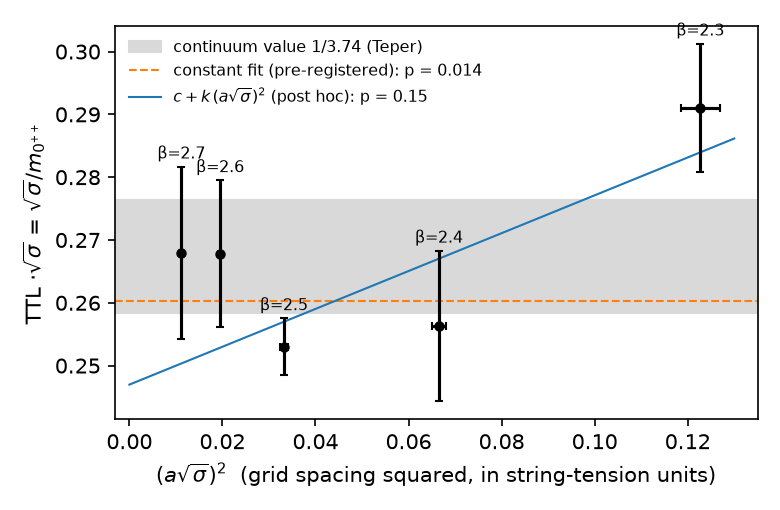
\includegraphics[width=0.72\linewidth]{fig-ttl.png}
\caption{The existence TTL in physical units at five grid spacings. Dashed: the pre-registered constant fit (fails, $p=0.014$). Solid: the
separately pre-registered post-hoc fit with an $a^2$ term ($p=0.15$). Grey: the continuum value from the literature.}\label{fig:ttl}
\end{figure}

\subsection{Test 4: do the twists carry the string tension?}

\lean{twisted\_balanced} shows that a network can pass every local check and still be off around a large loop. In SU(2) such global twists
are \emph{centre vortices}, and lattice work since 1997 finds that they carry most of the string tension~\cite{ddfgo97,dfde99}. The test, in
DMP's terms: are the twists what keeps IM within reach? Method: fix each configuration to maximal centre gauge, project each link to its
centre element $Z=\mathrm{sign}(\tfrac12\mathrm{tr}\,U)$, and compare Creutz ratios of the full links ($\chi_\text{full}$), the projected links
($\chi_\text{proj}$) and the links with vortices removed ($U'=ZU$, $\chi_\text{removed}$). A control projects without gauge fixing.

At $\beta=2.3$ ($12^4$, 100 configurations) the pre-registered test \textbf{fails}: at $R=3$, $\chi_\text{proj}/\chi_\text{full}=0.68$
(the criterion asked for agreement within 30\,\%) and removal leaves 34\,\%; at $R=4$ both criteria pass ($0.81\pm0.06$; $0.07\pm0.04$). The
control also fails formally: the projected loops without gauge fixing are 600 times smaller than with it, but at this statistical precision
not zero within 2 errors. The likely cause of the main failure is the choice of comparison, not the vortices: $\chi_\text{full}$ still falls
with $R$ (0.214, 0.184) because small Wilson loops carry short-distance terms on top of the string tension, while $\chi_\text{proj}$ is flat
(0.145, 0.149). The standard comparison is with the asymptotic string tension, which we had measured independently from torelons. We
pre-registered that comparison as a labelled post-hoc follow-up at $R=4$ and $5$, before looking at the $\beta=2.4$ run. At $\beta=2.3$
(not blind) it passes: $\chi_\text{proj}/\sigma a^2=1.21\pm0.05$ and $1.18\pm0.08$, and $\chi_\text{removed}$ is consistent with zero
(Figure~\ref{fig:vortex}). At $\beta=2.4$ (blind): \pending{vortex $\beta=2.4$ result}.

\begin{figure}[h]\centering
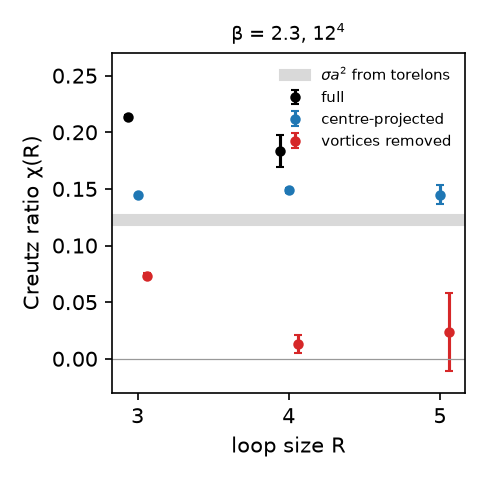
\includegraphics[width=0.6\linewidth]{fig-vortex.png}
\caption{Creutz ratios of the full links, the centre-projected links and the links with vortices removed, against loop size. Grey: the
string tension $\sigma a^2$ from torelons (an independent measurement).}\label{fig:vortex}
\end{figure}

\subsection{Test 5: the flux tube's L\"uscher term}

A closed flux tube of length $L$ vibrates in the two transverse directions, and its zero-point energy gives
$E(L)=\sigma L-\pi/(3L)+O(L^{-3})$~\cite{luscher81}. The coefficient $\pi/3$ is universal (it does not depend on the gauge group), and
lattice work has confirmed it~\cite{lw02}. We pre-registered a measurement at $\beta=2.3$ with boxes $L=6$ to $14$: pass if the fitted
coefficient agrees with $\pi/3$ within 2 errors with $p>0.05$. \pending{L\"uscher result}.

\subsection{What the numbers say}

Our code reproduces the known picture: in grid units the gap shrinks as the grid gets finer, in physical units it stays at the literature
value within errors once discretisation effects are accounted for; light is massless; centre vortices carry the string tension when compared
with the asymptotic string tension. The three failures are of the analysis rules we fixed in advance (a too-simple window, a constant fit
that ignored discretisation errors, a comparison with small-loop Creutz ratios), each identified and followed up openly. None of this is
evidence about the continuum beyond what the literature already has.

%=====================================================================================================================================
\section{Formal results independent of DMP}\label{sec:formal}

\subsection{The strong-coupling area law in Lean}

\paragraph{Statement.} For SU(2) with normalised Haar measure on the periodic lattice $(\mathbb Z/N\mathbb Z)^d$, Wilson weight
$\exp(\beta\sum_p\mathrm{Re\,tr}\,U_p)$ (this $\beta$ is half the standard SU(2) $\beta$), $\beta\ge0$ with $e^{2\beta}-1\le1/(4e^{16d+1}(16d+1)^4)$, and an $R\times T$ rectangular loop $C$
($1\le R,T<N$), the partition function is non-zero and
\[
|\langle W_C\rangle|\;\le\;2\,e^{16d(R+T)}\,\bigl(e^{16d+1}(e^{2\beta}-1)\bigr)^{A/2},\qquad A=\min(RT,\,N^2-RT)
\]
(\lean{wilson\_area\_law\_SU2}; for U($n$) the same with $e^{n\beta}-1$ and the factor $n$, \lean{wilson\_area\_law\_Un}). The base of the
power is below one throughout the allowed range, so the bound falls exponentially with the area: confinement at strong coupling.

\paragraph{Proof route.} (1) Expand each plaquette weight around its Haar mean, so the expectation becomes a ratio of sums over plaquette
sets. (2) Sets that share no link factorise (independence under the product measure). (3) Split each term into even and odd parts under
multiplying a link by the centre element $-1$; a term integrates to zero against the Wilson loop unless every link is covered an even number
of times by the loop and the odd plaquettes together (centre parity). (4) Any such odd set has at least $A$ plaquettes in the loop's plane,
by projecting to the plane and summing the parity condition (a minimal-area lemma). (5) Control the remaining sums with the Koteck\'y--Preiss
cluster expansion from the \texttt{balaban-lean} library~\cite{balabanlean}. All of it is finite: finite lattice, finite sums, no limits.

\paragraph{Status and prior work.} The build succeeds with no \lean{sorry}, and \lean{\#print axioms} on the final theorems shows only
Lean's standard axioms (\lean{propext}, \lean{Classical.choice}, \lean{Quot.sound}). The window of $\beta$ is tiny (for $d=4$, $\beta$ below
about $4\times10^{-37}$), as is typical of cluster-expansion constants that have not been optimised. The mathematics is Osterwalder and
Seiler's~\cite{os78}, and ours is not the first formalisation: a general SU($N$) area law was formalised before us
(\texttt{bharathsrivats/fisher-lorentz-formalization}, \lean{area\_law\_general}, which we checked has no \lean{sorry}), and another project
claims one (\texttt{lluiseriksson/THE-ERIKSSON-PROGRAMME}, not checked). Ours is an independent proof by a different route (cluster expansion
plus centre parity plus minimal area). It also fills a gap in the \texttt{lgt} library~\cite{lgt}, whose Wilson-loop file is a stub.

\subsection{Sharper influence bounds for \texttt{lgt}'s Dobrushin argument}

The \texttt{lgt} library proves exponential decay of correlations for U($n$) lattice gauge theory at strong coupling by Dobrushin's
uniqueness method~\cite{lgt}: each link's conditional law depends weakly on each neighbour, with influence at most $1-e^{-4n\beta}$, and the
sum over $8(d-1)$ neighbours is below one (roughly $\beta<1/(32n(d-1))$ in its normalisation). The influence bound can be sharpened in
three steps, in decreasing order of rigour.

\begin{lemma}
If $\mu\ll\nu$ are probability measures and $g=d\mu/d\nu$ takes values in $[m,M]$ with $M/m\le R$, then
$\mathrm{TV}(\mu,\nu)\le(\sqrt R-1)/(\sqrt R+1)=\tanh(\tfrac14\ln R)$.
\end{lemma}
\begin{proof}
$\mathrm{TV}=\int(g-1)_+\,d\nu$. For fixed $m,M$ with $\int g\,d\nu=1$ this is largest when $g$ takes only the values $M$ (on $\nu$-mass $p$) and
$m$, so $p=(1-m)/(M-m)$ and $\mathrm{TV}=(M-1)(1-m)/(M-m)$. With $M=Rm$ this is maximal at $m=1/\sqrt R$, where it equals
$(\sqrt R-1)/(\sqrt R+1)$.
\end{proof}

(i) \texttt{lgt}'s existing cylinder-ratio hypothesis bounds the density to $[e^{-C},e^{C}]$ with $C=4n\beta$, so $R=e^{2C}$ and the lemma gives
influence $\le\tanh(2n\beta)$: a factor 2 with the same hypothesis. (ii) Changing a neighbour changes one plaquette's cost, which lies in a
range of width $2n\beta$ for every value of the link, so the log-density oscillates by at most $4n\beta$ and the influence is at most
$\tanh(n\beta)$: a factor 4, which needs the cylinder-ratio lemma restated with the oscillation. (iii) \texttt{lgt}'s own comment notes that the
tight neighbour count is $6(d-1)$, not $8(d-1)$. Numerically, the exact single-link influence has a closed form at the worst case we found
(a ratio of a modified Struve to a modified Bessel function: $L_0(\beta)/I_0(\beta)$ for U(1), $L_1(\beta)/I_1(\beta)$ for SU(2)), giving
factors of about 8 and 12 over \texttt{lgt}'s threshold; that the worst case is the one found is not proved. For SU(2) the curvature method of
Shen, Zhu and Zhu~\cite{szz} already reaches further than every rigorous row here ($\beta<1/(4(d-1))$ in the standard normalisation); the
improvements matter for U(1) and U($n$), which it does not cover, and for \texttt{lgt}'s own route. All of these thresholds are far below the
physical region ($\beta\approx2.3$ for SU(2)).

%=====================================================================================================================================
\section{What this does not show, and what might}\label{sec:outlook}

The reading does not prove a mass gap, and it does not make one more likely. What it shows is where the problem sits in a second vocabulary:
DMP takes bounded nodes and bounded reach as axioms, and Yang--Mills has to derive them. The photon test then says which kinds of argument
cannot work (anything that does not use the non-commutativity of the gauge group, and any layered argument that cannot resolve
$10^{-11}$ per layer).

Three directions would move the work. \emph{First}, the improvements of \S\ref{sec:formal} are ready to be proposed to \texttt{lgt}: the lemma
of step (i) is a local change to one proof. \emph{Second}, the vortex and TTL follow-ups at finer grids, with continuum extrapolation, would
turn the post-hoc checks into pre-registered tests over a range of scales. \emph{Third}, and closest to the first author's reading that a
DMP-complete system ``self-certifies'' its existence from consistency alone: bootstrap methods derive rigorous bounds on a theory from
consistency conditions such as positivity, without constructing it~\cite{prv19}, and they have been applied to lattice Yang--Mills
itself~\cite{kz23}. Whether DMP's consistency conditions add anything to those is an open question that this paper does not answer.

%=====================================================================================================================================
\section*{Contributions and use of AI}\addcontentsline{toc}{section}{Contributions and use of AI}

Steven Hrovat wrote DMP and the GUID series, set the direction of this work, and contributed the readings quoted in
\S\S\ref{sec:dmp}--\ref{sec:reach} (the IM/payload classification, the reach reading of Axiom 1, the existence TTL, and the hosting
framing, all on 21 November 2026). Claude (Anthropic; Claude Opus 5.5 in Claude Code) wrote the code, ran the computations, wrote the
proofs and the text, and checked the claims against the literature. Parts of the Lean area-law proof (the cluster-ratio bound, the
minimal-area lemma, the assembly and the concrete groups) were written by Claude subagents and checked by the main session (build, scan for
escape hatches, axioms). A Claude Fable 5.2 subagent reviewed the claims adversarially before this draft; its corrections are applied
(among them: the reach chain is a restatement, not a derivation; the SU(3)/SU(2) layer ratio is an identity, not a test).

\section*{Reproducibility}\addcontentsline{toc}{section}{Reproducibility}

Everything is in the \texttt{gravity} repository under \texttt{docs/mass-gap/}; the DMP-side Lean theorems are in \texttt{evidence/Dmp/}
(285 theorems, checked by \texttt{evidence/tools/check.sh} on Lean 4.34). The area law is in \texttt{docs/mass-gap/arealaw/} (Lean 4.35.0-rc2,
built against \texttt{balaban-lean}; \texttt{sync-build.sh}). Pre-registrations are the \texttt{PREREG*.md} files next to the scripts, with
their results appended; their commit times are in the history. Stored results: \texttt{docs/mass-gap/results/}. Figures:
\texttt{paper/figures.py}. The numbers quoted in this paper are re-derived from the stored results by \texttt{paper/checks.py}.

%=====================================================================================================================================
\begin{thebibliography}{99}\small
\bibitem{balabanlean} \texttt{scottnarmstrong/balaban-lean}, Lean formalisation of polymer expansions (Apache-2.0),
  \url{https://github.com/scottnarmstrong/balaban-lean}.
\bibitem{cns25} S.~Cao, R.~Nissim, S.~Sheffield, arXiv:2505.16585 (2025).
\bibitem{ddfgo97} L.~Del Debbio, M.~Faber, J.~Greensite, \v{S}.~Olejn\'ik, Phys.\ Rev.\ D 55 (1997) 2298.
\bibitem{dfde99} P.~de Forcrand, M.~D'Elia, Phys.\ Rev.\ Lett.\ 82 (1999) 4582.
\bibitem{dmp} S.~Hrovat, DMP, the Dark Matter Protocol, version 0.9.9 (2026), vendored in the \texttt{gravity} repository as \texttt{vendor/dmp}.
\bibitem{fs82} J.~Fr\"ohlich, T.~Spencer, Commun.\ Math.\ Phys.\ 83 (1982) 411.
\bibitem{gm82} M.~G\"opfert, G.~Mack, Commun.\ Math.\ Phys.\ 82 (1982) 545.
\bibitem{guidv7} S.~Hrovat, Claude, GUID v7: From Inflation to the Standard Model, read through the axioms of DMP (2026),
  \texttt{gravity/docs/guid-v7}.
\bibitem{guth} A.~Guth, Phys.\ Rev.\ D 21 (1980) 2291.
\bibitem{itoseiler} K.~R.~Ito, E.~Seiler, arXiv:0711.4930, arXiv:0803.3019.
\bibitem{jaffewitten} A.~Jaffe, E.~Witten, Quantum Yang--Mills theory, Clay Mathematics Institute problem description (2000).
\bibitem{kadanoff} L.~P.~Kadanoff, Ann.\ Phys.\ 100 (1976) 359.
\bibitem{kz23} V.~Kazakov, Z.~Zheng, Bootstrap for lattice Yang--Mills theory, Phys.\ Rev.\ D 107 (2023) L051501, arXiv:2203.11360.
\bibitem{lgt} M.~R.~Douglas et al., \texttt{lgt}, Lean formalisation of lattice gauge theory, \url{https://github.com/mrdouglasny/lgt}.
\bibitem{luscher81} M.~L\"uscher, Nucl.\ Phys.\ B 180 (1981) 317.
\bibitem{lw02} M.~L\"uscher, P.~Weisz, JHEP 07 (2002) 049.
\bibitem{migdal} A.~A.~Migdal, Sov.\ Phys.\ JETP 42 (1976) 413.
\bibitem{openai2026} OpenAI, Lean-checked construction of four-dimensional Yang--Mills theory as a lattice scaling limit, and the
  assessment of the review committee chaired by D.~Gross (validated 10 November 2026).
\bibitem{os78} K.~Osterwalder, E.~Seiler, Ann.\ Phys.\ 110 (1978) 440.
\bibitem{prv19} D.~Poland, S.~Rychkov, A.~Vichi, Rev.\ Mod.\ Phys.\ 91 (2019) 015002.
\bibitem{szz} H.~Shen, R.~Zhu, X.~Zhu, arXiv:2204.12737.
\bibitem{teper} M.~Teper, hep-th/9812187.
\bibitem{tomboulis} E.~T.~Tomboulis, arXiv:0707.2179.
\bibitem{wilson74} K.~G.~Wilson, Phys.\ Rev.\ D 10 (1974) 2445.
\end{thebibliography}

\end{document}
